
\begin{frame}
  \frametitle{Research Overview}
  \begin{minipage}{0.58\textwidth}
    \textit{Given the expected tradeoff between time and information:} \\~\\
    How does the ability to determine forensic-relevant spent nuclear fuel
    attributes using machine learning techniques degrade as less information is
    available?
  \end{minipage}%
  \hfill
  \begin{minipage}{0.38\textwidth}
    \begin{figure}
      \centering
      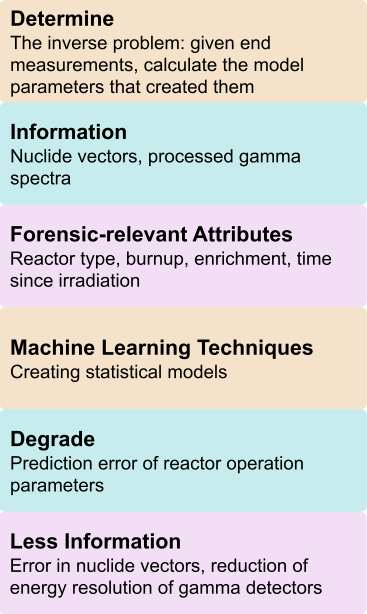
\includegraphics[height=0.85\textheight]{./figures/overview.png}
    \end{figure}
  \end{minipage}
\end{frame}

\begin{frame}
  \frametitle{Developing a Computational Methodology} %Research Overview
  \begin{figure}[h!]
    \centering
    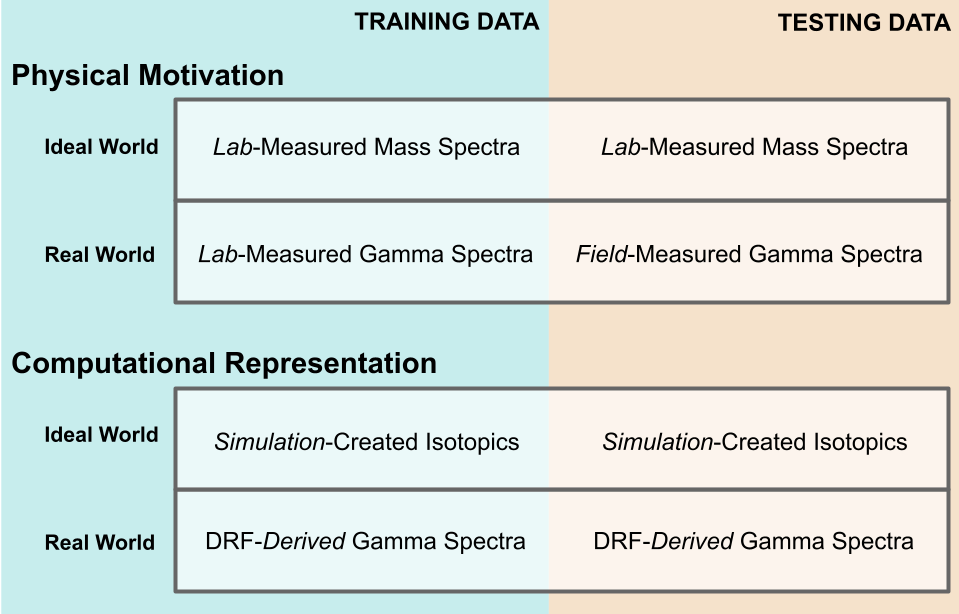
\includegraphics[width=0.9\textwidth]{./figures/project_design.png}
  \end{figure}
\end{frame}

\begin{frame}
  \frametitle{Developing a Statistical Methodology}
  \begin{adjustwidth}{-10pt}{-10pt}
  \begin{minipage}{0.5\textwidth}
    \begin{figure}
      \centering
      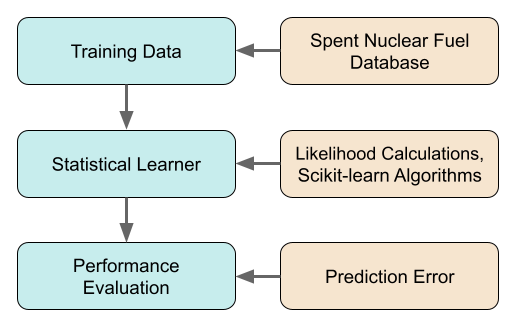
\includegraphics[width=\textwidth]{./figures/meth_pres.png}
    \end{figure}
  \end{minipage}%
  %\hfill
  \begin{minipage}{0.533\textwidth}
    \begin{itemize}
      \item Training Data: SNF recipes from SCALE/ORIGEN-ARP \cite{scale, origen}
      \item Statistical Methods
        \begin{itemize}
          \item Scikit-learn algorithms (kNN \& Decision Trees) \cite{scikit}
          \item Maximum log-likelihood calculation method \cite{mll_method, mll_sensitivity}
        \end{itemize}
      \item Performance
        \begin{itemize}
          \item Test cases from SFCOMPO \cite{sfcompo}
          \item Prediction error analysis
        \end{itemize}
    \end{itemize}
  \end{minipage}
  \end{adjustwidth}
\end{frame}


